% !TEX root = smc_bandits.tex

We assess the impact of Monte Carlo sample size $M$ in the performance of the proposed SMC-based Bayesian MAB policies:
In Figure~\ref{fig:dynamic_bandits_linearGaussian_a_M}, we present results for Scenario A defined by Equation~\eqref{eq:linear_mixing_dynamics_a},
for a realization of expected rewards as depicted in Figure~\ref{fig:linear_mixing_dynamics_a_gaussian};
In Figure~\ref{fig:dynamic_bandits_linearGaussian_b_M}, we  present results for Scenario B defined by Equation~\eqref{eq:linear_mixing_dynamics_b}, 
with a realization of expected rewards as depicted in Figure~\ref{fig:linear_mixing_dynamics_b_gaussian}.

% Scenario A
\begin{figure}[!h]
	\centering
	\begin{subfigure}[b]{0.45\textwidth}
		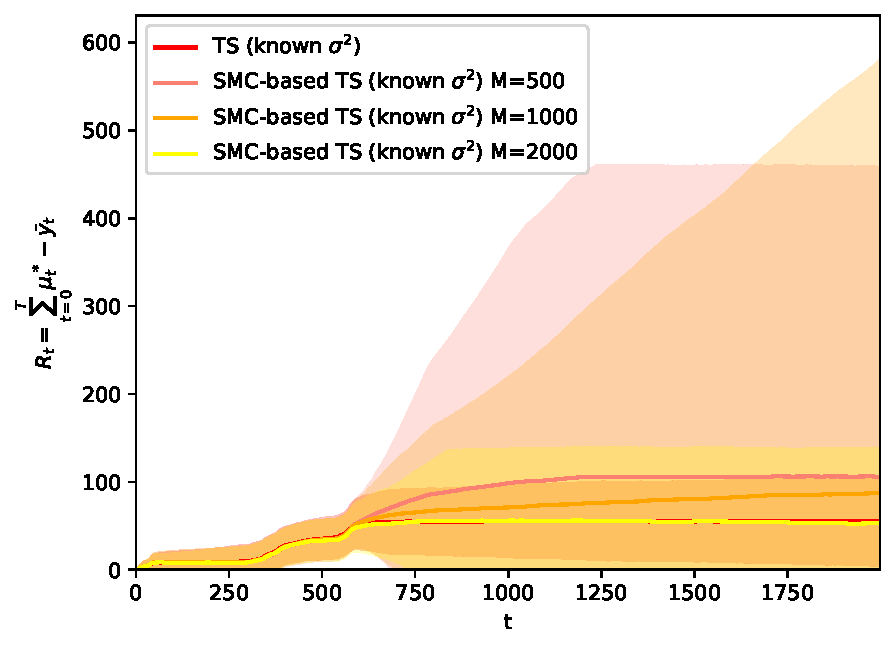
\includegraphics[width=\textwidth]{./fods_figs/dynamic/linearGaussian/a_selectedM_cumulative_regret_dknown_ts_knownsigma}
		\caption{Cumulative regret for SMC-based TS in scenario A: known dynamic parameters.}
		\label{fig:dynamic_bandits_linearGaussian_a_ts_dknown_knownsigma_M}
	\end{subfigure}\qquad
	\begin{subfigure}[b]{0.45\textwidth}
		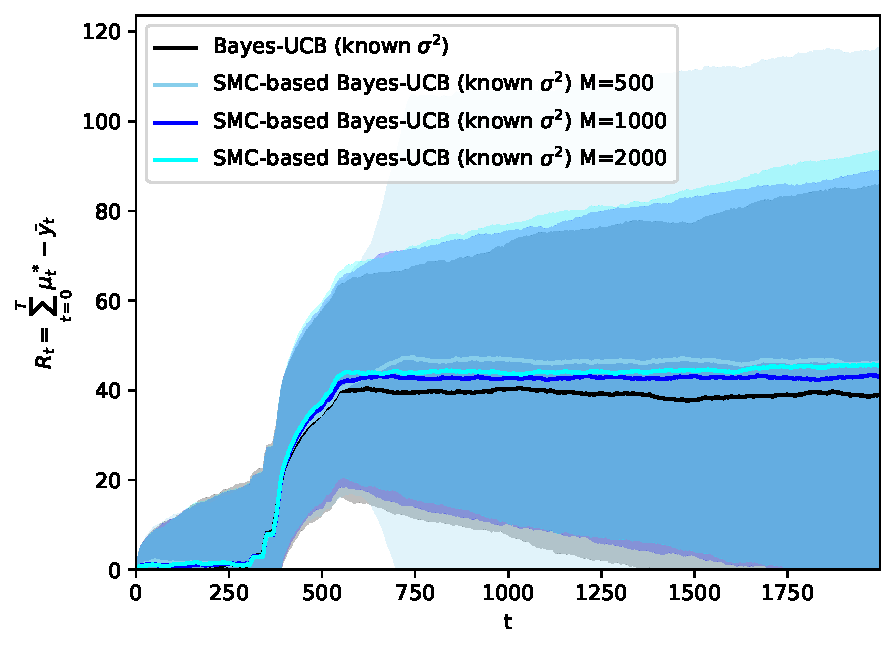
\includegraphics[width=\textwidth]{./fods_figs/dynamic/linearGaussian/a_selectedM_cumulative_regret_dknown_bucb_knownsigma}
		\caption{Cumulative regret for SMC-based Bayes-UCB in scenario A: known dynamic parameters.}
		\label{fig:dynamic_bandits_linearGaussian_a_bucb_dknown_knownsigma_M}
	\end{subfigure}
	
	\begin{subfigure}[b]{0.45\textwidth}
		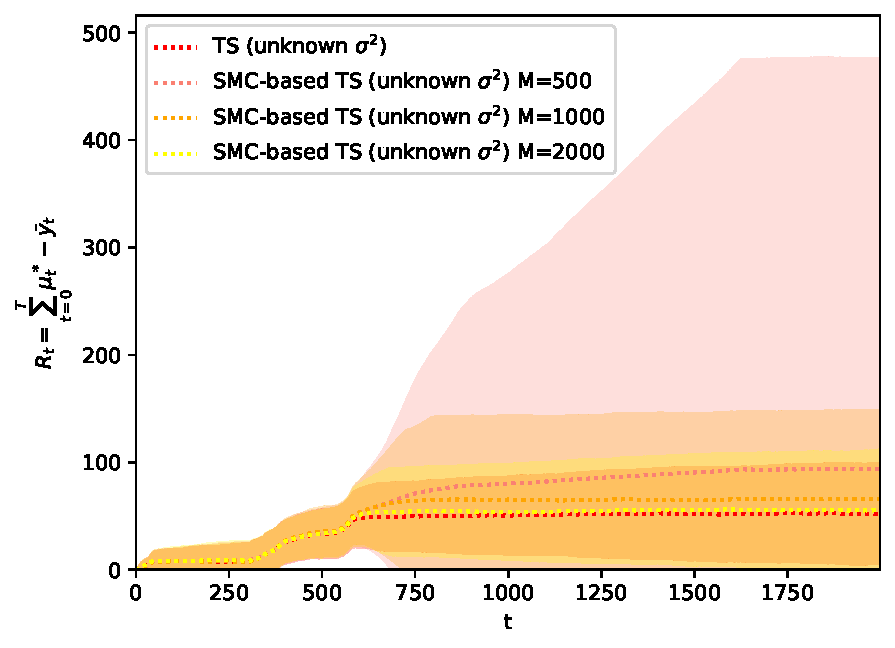
\includegraphics[width=\textwidth]{./fods_figs/dynamic/linearGaussian/a_selectedM_cumulative_regret_dknown_ts_unknownsigma}
		\caption{Cumulative regret for SMC-based TS in scenario A: known dynamic parameters, unknown $\sigma_a^2, \forall a$.}
		\label{fig:dynamic_bandits_linearGaussian_a_ts_dknown_unknownsigma_M}
	\end{subfigure}\qquad
	\begin{subfigure}[b]{0.45\textwidth}
		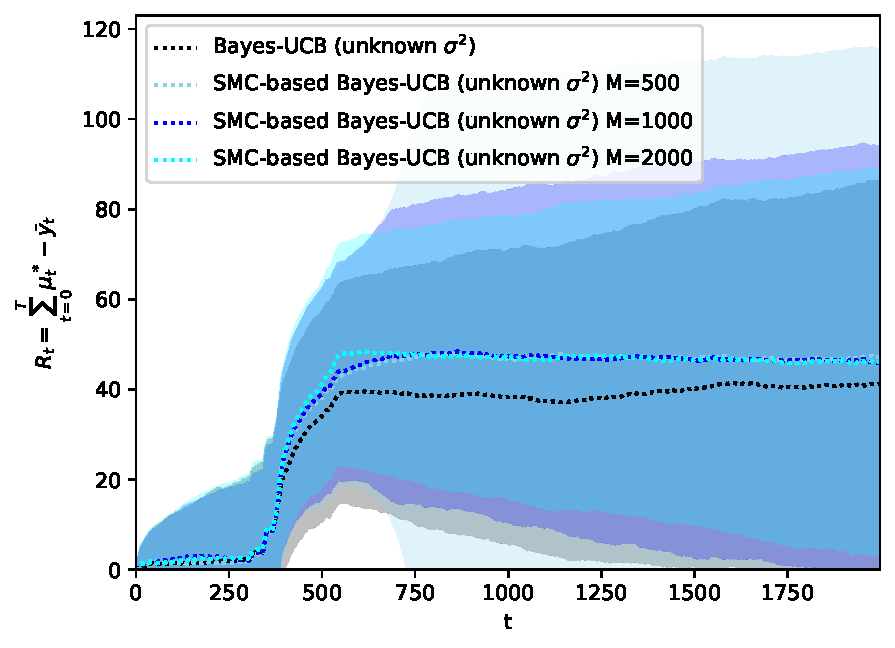
\includegraphics[width=\textwidth]{./fods_figs/dynamic/linearGaussian/a_selectedM_cumulative_regret_dknown_bucb_unknownsigma}
		\caption{Cumulative regret for SMC-based Bayes-UCB in scenario A: known dynamic parameters, unknown $\sigma_a^2, \forall a$.}
		\label{fig:dynamic_bandits_linearGaussian_a_bucb_dknown_unknownsigma_M}
	\end{subfigure}
	
		\begin{subfigure}[b]{0.45\textwidth}
		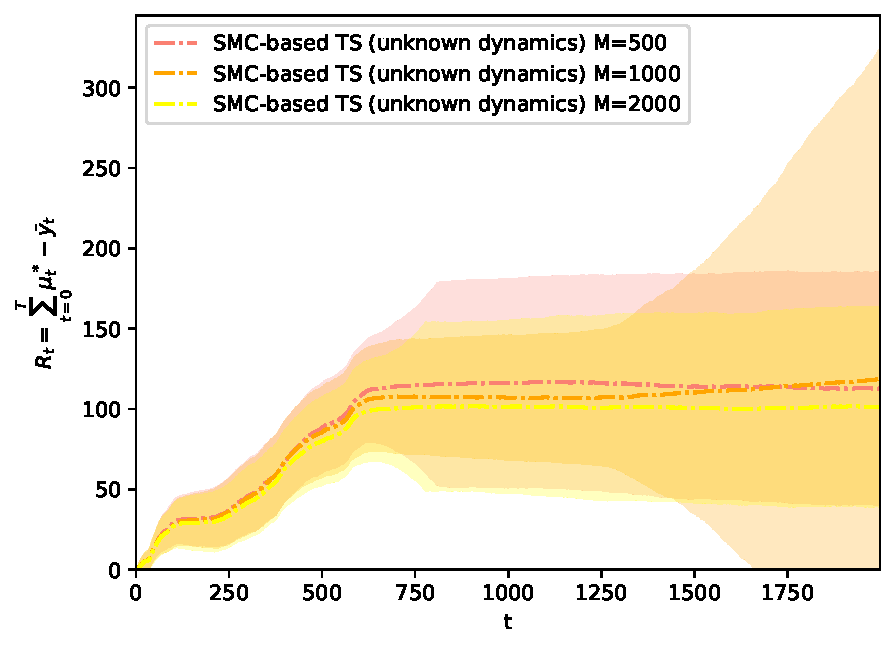
\includegraphics[width=\textwidth]{./fods_figs/dynamic/linearGaussian/a_selectedM_cumulative_regret_dunknown_ts}
		\caption{Cumulative regret for SMC-based TS in scenario A: unknown dynamic parameters $L_a,\Sigma_a,\sigma_a^2, \forall a$.}
		\label{fig:dynamic_bandits_linearGaussian_a_ts_dunknown_M}
	\end{subfigure}\qquad
	\begin{subfigure}[b]{0.45\textwidth}
		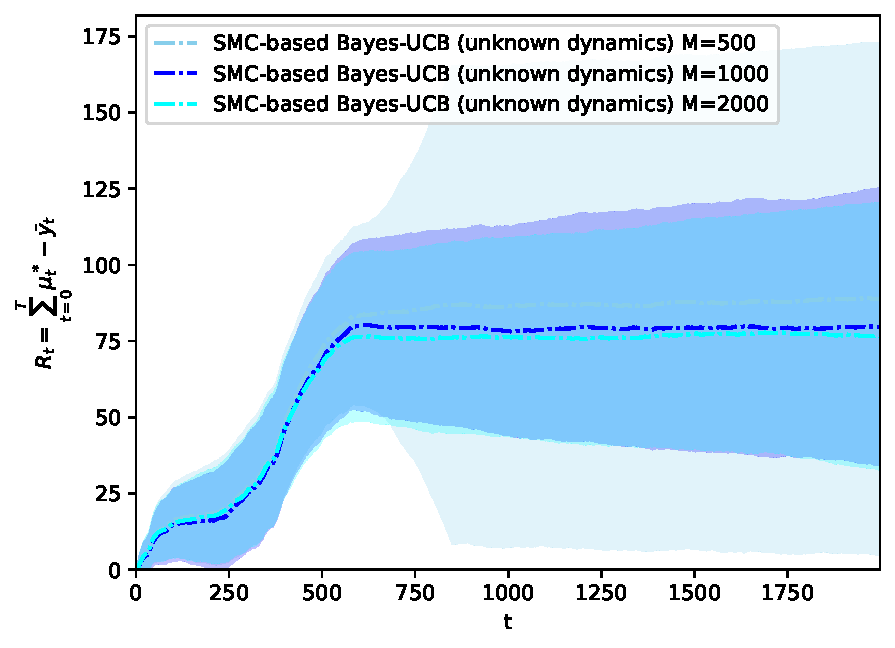
\includegraphics[width=\textwidth]{./fods_figs/dynamic/linearGaussian/a_selectedM_cumulative_regret_dunknown_bucb}
		\caption{Cumulative regret for SMC-based Bayes-UCB in scenario A: unknown dynamic parameters $L_a,\Sigma_a,\sigma_a^2, \forall a$.}
		\label{fig:dynamic_bandits_linearGaussian_a_bucb_dunknown_M}
	\end{subfigure}

	\caption{
		Mean regret (standard deviation shown as the shaded region) in contextual, linear Gaussian bandit Scenario A
		described in Equation~\eqref{eq:linear_mixing_dynamics_a}.
		SMC-based policies' averaged cumulative regret is robust to different Monte Carlo sample sizes $M$,
		which impacts mostly the performance variability for $M=500$. 
	}
	\label{fig:dynamic_bandits_linearGaussian_a_M}
\end{figure}

% Scenario B
\begin{figure}[!h]
	\centering
	\begin{subfigure}[b]{0.45\textwidth}
		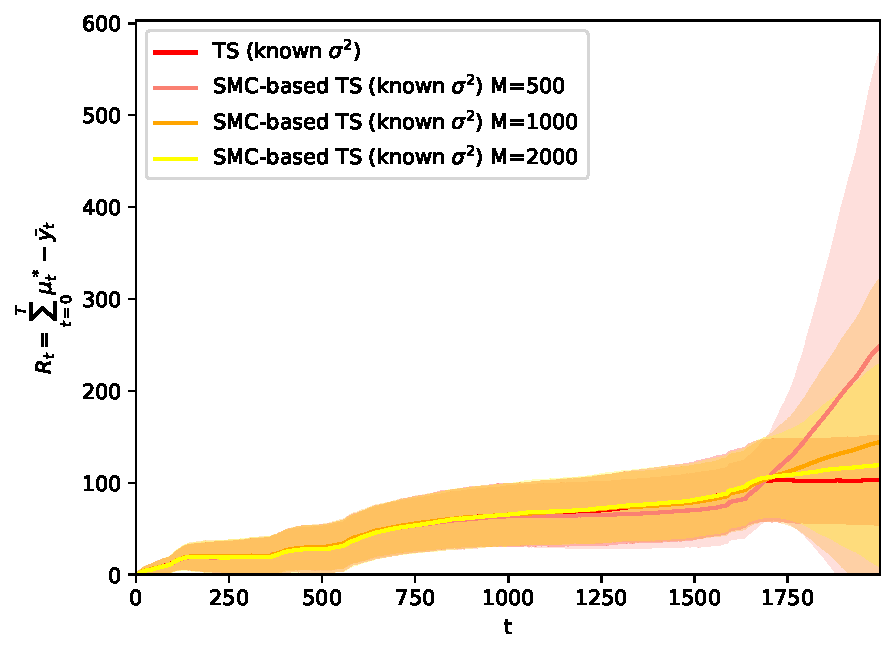
\includegraphics[width=\textwidth]{./fods_figs/dynamic/linearGaussian/b_selectedM_cumulative_regret_dknown_ts_knownsigma}
		\caption{Cumulative regret for SMC-based TS in scenario B: known dynamic parameters.}
		\label{fig:dynamic_bandits_linearGaussian_b_ts_dknown_knownsigma_M}
	\end{subfigure}\qquad
	\begin{subfigure}[b]{0.45\textwidth}
		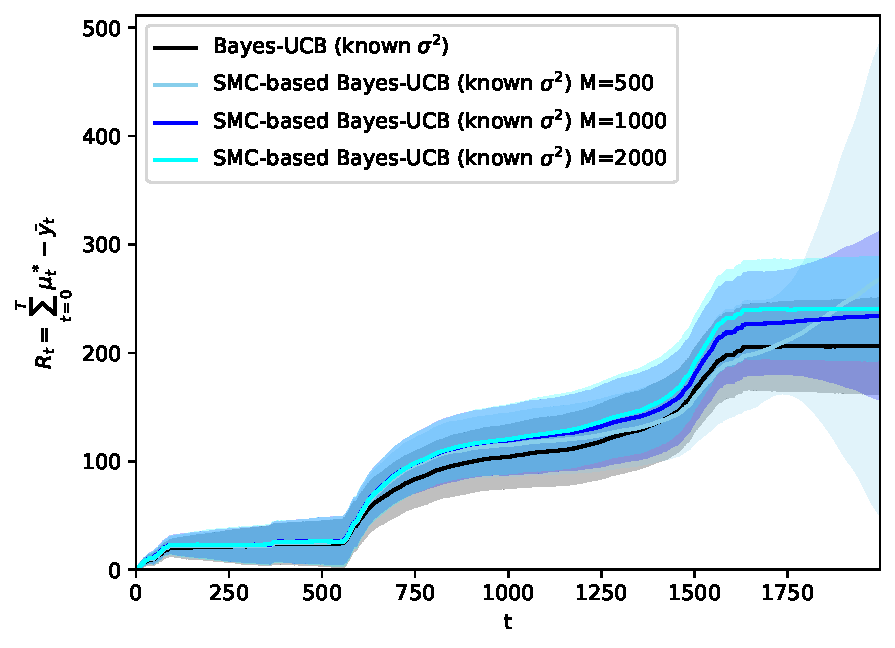
\includegraphics[width=\textwidth]{./fods_figs/dynamic/linearGaussian/b_selectedM_cumulative_regret_dknown_bucb_knownsigma}
		\caption{Cumulative regret for SMC-based Bayes-UCB in scenario B: known dynamic parameters.}
		\label{fig:dynamic_bandits_linearGaussian_b_bucb_dknown_knownsigma_M}
	\end{subfigure}
	
	\begin{subfigure}[b]{0.45\textwidth}
		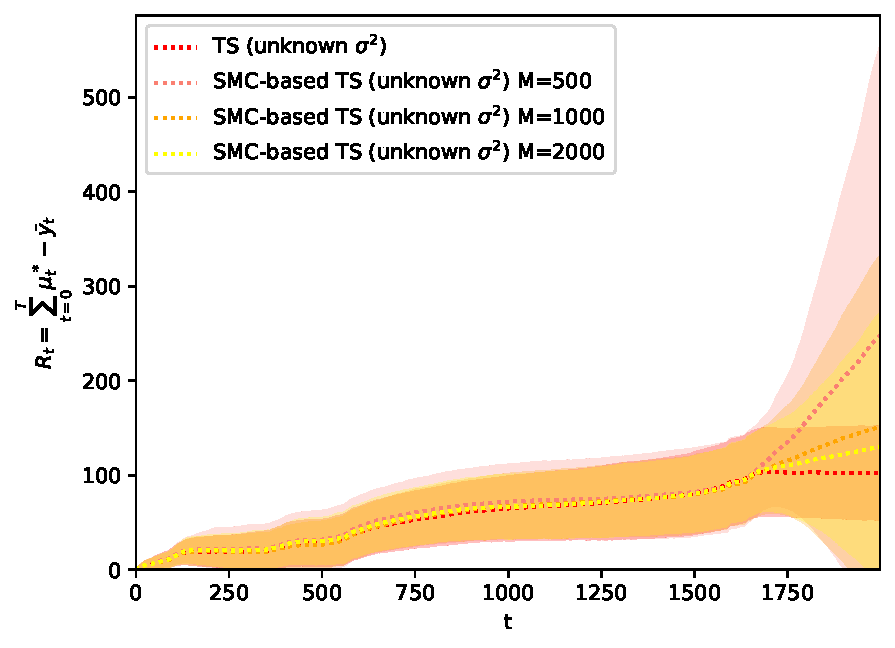
\includegraphics[width=\textwidth]{./fods_figs/dynamic/linearGaussian/b_selectedM_cumulative_regret_dknown_ts_unknownsigma}
		\caption{Cumulative regret for SMC-based TS in scenario B: known dynamic parameters, unknown $\sigma_a^2, \forall a$.}
		\label{fig:dynamic_bandits_linearGaussian_b_ts_dknown_unknownsigma_M}
	\end{subfigure}\qquad
	\begin{subfigure}[b]{0.45\textwidth}
		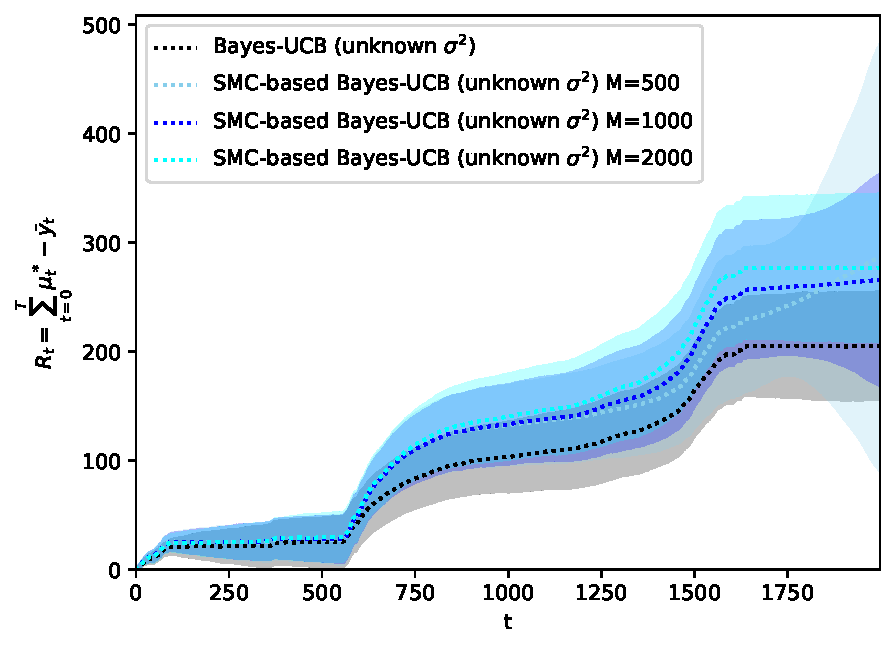
\includegraphics[width=\textwidth]{./fods_figs/dynamic/linearGaussian/b_selectedM_cumulative_regret_dknown_bucb_unknownsigma}
		\caption{Cumulative regret for SMC-based Bayes-UCB in scenario B: known dynamic parameters, unknown $\sigma_a^2, \forall a$.}
		\label{fig:dynamic_bandits_linearGaussian_b_bucb_dknown_unknownsigma_M}
	\end{subfigure}
	
	\begin{subfigure}[b]{0.45\textwidth}
		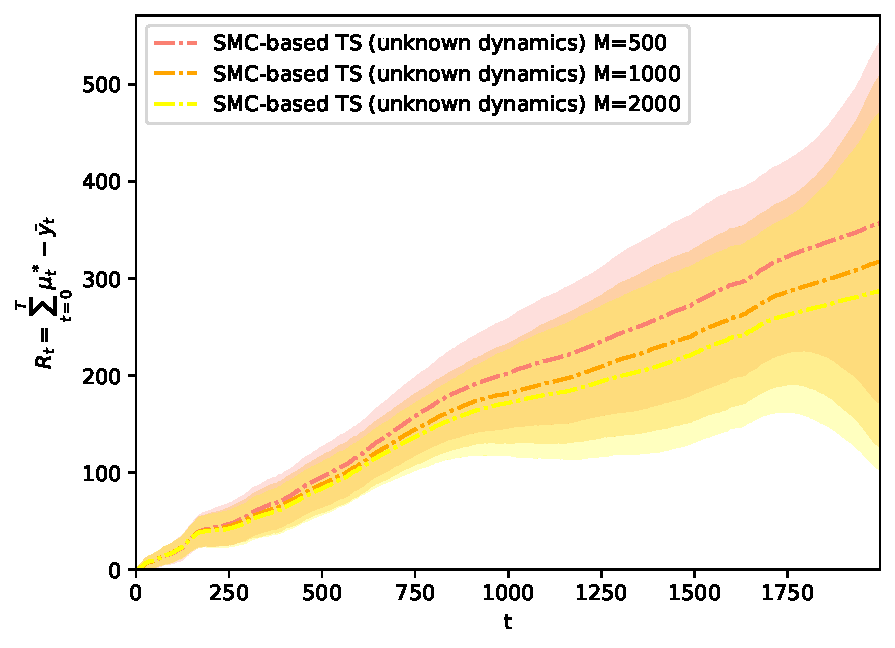
\includegraphics[width=\textwidth]{./fods_figs/dynamic/linearGaussian/b_selectedM_cumulative_regret_dunknown_ts}
		\caption{Cumulative regret for SMC-based TS in scenario B: unknown dynamic parameters $L_a,\Sigma_a,\sigma_a^2, \forall a$.}
		\label{fig:dynamic_bandits_linearGaussian_b_ts_dunknown_M}
	\end{subfigure}\qquad
	\begin{subfigure}[b]{0.45\textwidth}
		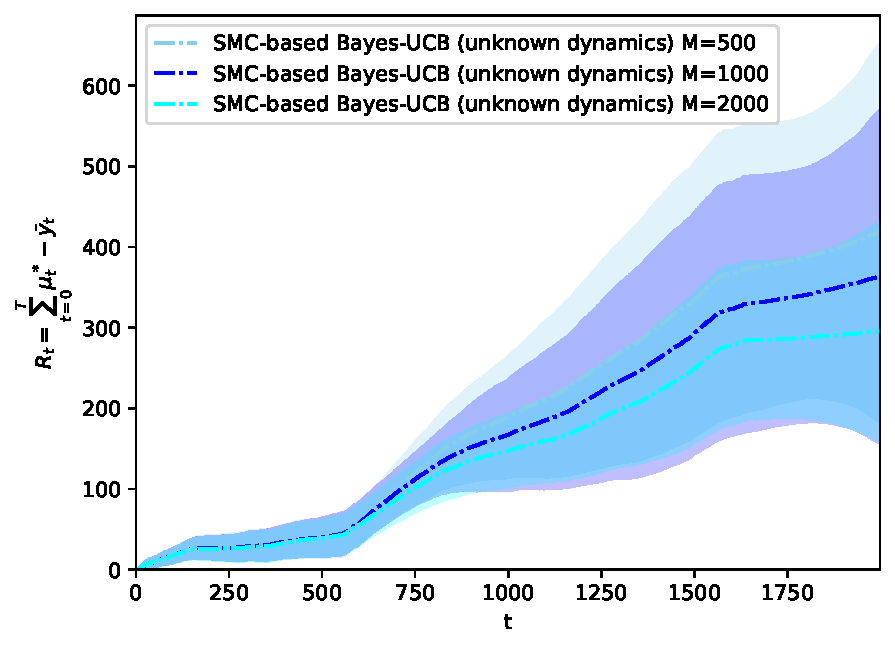
\includegraphics[width=\textwidth]{./fods_figs/dynamic/linearGaussian/b_selectedM_cumulative_regret_dunknown_bucb}
		\caption{Cumulative regret for SMC-based Bayes-UCB in scenario B: unknown dynamic parameters $L_a,\Sigma_a,\sigma_a^2, \forall a$.}
		\label{fig:dynamic_bandits_linearGaussian_b_bucb_dunknown_M}
	\end{subfigure}
	
	\caption{
		Mean regret (standard deviation shown as the shaded region) in contextual, linear Gaussian bandit Scenario B
		described in Equation~\eqref{eq:linear_mixing_dynamics_b}.
		SMC-based policies' averaged cumulative regret is robust to different Monte Carlo sample sizes $M$,
		which impacts mostly the performance variability for $M=500$ ---specially so when optimal arm swaps occur later in time.
	}
	\label{fig:dynamic_bandits_linearGaussian_b_M}
\end{figure}